\chapter{Contenido didáctico}
\label{chap:contenido_didactico}

\lettrine{U}{na} importante parte de este proyecto es la forma en la que sirve para explicar el funcionamiento del mismo, así como realizar demostraciones prácticas de dicho funcionamiento.

Para este cometido se desarrolla una aplicación web desde la cual se podrán ejecutar ....

\section{Requisitos}
Los requisitos son relacionados con docencia, utilidad, tendrán vídeos, será sencillo de usar etc......

\subsection{Requisitos funcionales y no funcionales}
Requisitos blabla

\subsection{Prerrequisitos}
\subsubsection{Netdata}
Netdata es el software de monitorización que nos permitirá obtener información del cluster en tiempo real, tanto en el \textit{Dashboard} web que se pone a disposición del usuario en el puerto 19999, como a través de la librería JavaScript que un programador puede importar en su propia página web.

Para emplear los datos que nos proporciona este software, primero debe instalarse y activarse en cada uno de los nodos del cluster, acción que se realiza con los comandos como usuario root.

\begin{lstlisting}[language=bash]
pacman -S netdata   # Se instala netdata
# Se activa netdata a través de todas las interfaces
sed -i 's/bind to = localhost/bind to = 0.0.0.0/g' /etc/netdata/netdata.conf
# Se activa e inicia netdata
systemctl enable --now netdata
\end{lstlisting}

\subsubsection{Dashboard}
Para desplegar el dashboard es necesario instalar npm y git en el nodo maestro:
\begin{lstlisting}[language=bash]
pacman -S npm git --needed      # como root
\end{lstlisting}

Tras ello se procede a desplegar la app
\begin{lstlisting}[language=bash]
# Se crea el directorio /clupiter_dashboard y se le dan permisos a mpiuser
mkdir /clupiter_dashboard
chown -R mpiuser:mpiuser /clupiter_dashboard

# Se inicia sesión como mpiuser
su - mpiuser
cd /clupiter_dashboard

# Se descarga la app y se entra al directorio del servidor
git clone https://github.com/forcegk/GEI_TFG.git
cd GEI_TFG/app/node/

# Se instalan las dependencias
npm install --only=production

# Y se ejecuta manualmente una vez para probar con
node ./index.js
\end{lstlisting}

Si todo ha funcionado correctamente se podrá acceder al \textit{Dashboard} en la dirección

\begin{figure}[H]
    \vspace{0.3cm}
    \centering
    \url{http://192.168.0.220:3000/monitoring.html}
\end{figure}

% TODO INSERTAR CAPTURA

\subsubsection{Unit de systemd}
Crear una unit de systemd es necesario para que el la página web se inicie con el nodo maestro. Realizar esto es una operación moderadamente sencilla (si bien no tan sencilla como podría ser en otros sistemas de init\footnote{\url{https://wiki.gentoo.org/wiki/Comparison_of_init_systems}}) 

La creación de la unit se realiza editando como usuario root el fichero \texttt{/etc/systemd/system/clupiter\_dashboard.service}:

\begin{lstlisting}[]
[Unit]
Description=Service for Clupiter Dashboard
After=network.target

[Service]
Type=simple
User=mpiuser
WorkingDirectory=/clupiter_dashboard/GEI_TFG/app/node
ExecStart=/usr/bin/node /clupiter_dashboard/GEI_TFG/app/node/index.js
Restart=on-failure

[Install]
WantedBy=multi-user.target
\end{lstlisting}

Tras la creación de la unit, se recarga el demonio de systemd, y se inicia el Dashboard, también como root:
\begin{lstlisting}[language=bash]
# Se reinicia el demonio
systemctl daemon-reload

# Se activa e inicia el servicio
systemctl enable --now clupiter_dashboard.service

# Se puede verificar el correcto inicio del servicio con
systemctl status clupiter_dashboard.service
\end{lstlisting}

Si todo ha funcionado correctamente, se debería ver la pantalla mostrada en la Figura \ref{fig:systemd_clupiter_dashboard} al ejecutar el último comando (de la cual se puede salir presionando la letra \texttt{q}).

\begin{figure}[H]
  \centering
  \vspace*{0.5cm}
  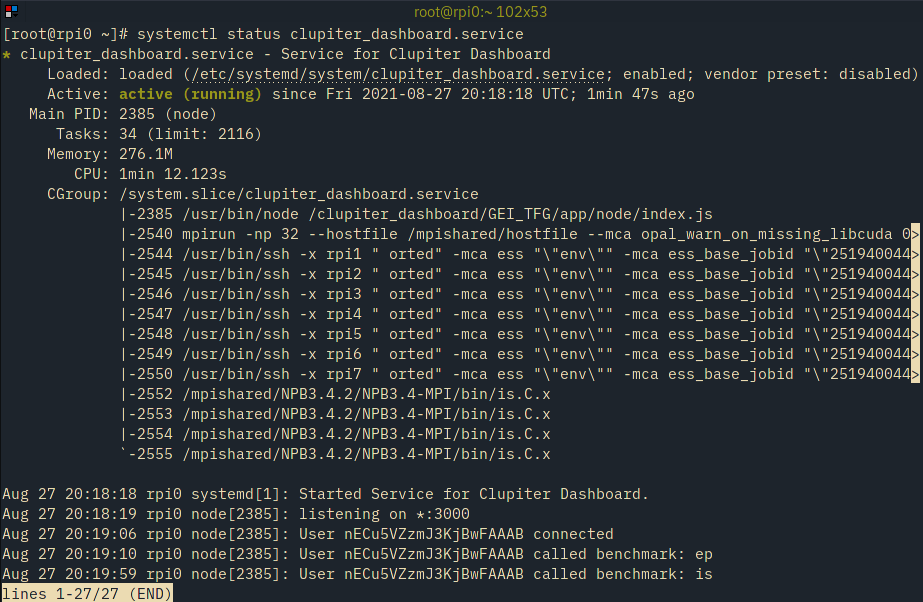
\includegraphics[width=0.9\textwidth]{img/systemd_clupiter_dashboard.png}
  \caption{Servicio \textit{Clupiter Dashboard} ejecutando un benchmark correctamente}
  \label{fig:systemd_clupiter_dashboard}
\end{figure}

\section{Diseño}
Se sigue un proceso de diseño mediante el uso de prototipos (\textit{mockups})... (TODO insertar escaneos de mockups en diseño)

\section{Funcionamiento}

TODO implementar botón de apagado
